\documentclass[11pt,a4paper]{article}
\usepackage{iftex}
\ifPDFTeX\usepackage[utf8]{inputenc}\fi
\usepackage[T1]{fontenc}
\usepackage[spanish,es-noshorthands]{babel}
\usepackage{mathptmx,textcomp,microtype}
\usepackage[margin=53pt,bottom=49pt]{geometry}
\usepackage{graphicx,tabularx,array,booktabs}
\usepackage[table]{xcolor}
\usepackage{titlesec}
\usepackage[hidelinks,unicode]{hyperref}
\hypersetup{pdftitle={Vía aplicación de movilidad Entrega 1},pdfauthor={Ruben Andres Szasz Szasz; Kilian Escudero Vizcaino; Ismael Ferrando Paulo}}
\graphicspath{{../03_Mockups/}}
\setlength{\parindent}{0pt}
\setlength{\parskip}{7pt}
\setlength{\tabcolsep}{6pt}
\renewcommand{\arraystretch}{1.15}
\newcolumntype{Y}{>{\raggedright\arraybackslash}X}
\titleformat{\section}{\fontsize{17}{20}\selectfont\bfseries}{\thesection.}{0.5em}{}
\titleformat{\subsection}{\fontsize{11.8}{15}\selectfont\bfseries}{}{0pt}{}
\titlespacing*{\section}{0pt}{14pt}{10pt}
\titlespacing*{\subsection}{0pt}{12pt}{7pt}
\pagestyle{plain}
\raggedbottom
\emergencystretch=1em
\begin{document}
\fontsize{10.8}{14.7}\selectfont
\begin{center}
{\fontsize{25}{30}\selectfont\bfseries Vía: aplicación de movilidad\par}
\vspace{7pt}
{\fontsize{18}{23}\selectfont\bfseries Especificación de requisitos y diseño inicial\par}
\vspace{11pt}
{\fontsize{12}{16}\selectfont Entrega 1\textperiodcentered{} EI1039 y EI1048\par}
\vspace{14pt}
Grado en Ingeniería Informática\textperiodcentered{} Universitat Jaume I\\
Curso 2026-2027\textperiodcentered{} 15 de octubre de 2026
\vspace{12pt}

Ruben Andres Szasz Szasz\\
Kilian Escudero Vizcaino\\
Ismael Ferrando Paulo
\end{center}
\vspace{14pt}
\textbf{Resumen}\par
Vía es una aplicación de movilidad para gestionar lugares y vehículos y calcular rutas. Se presentan seis requisitos funcionales, 26 historias de usuario y 52 escenarios con sus pruebas de aceptación. La propuesta se completa con nueve mockups, un spike que integra las tecnologías elegidas y la declaración de uso de IA generativa.

\vspace{10pt}
\textbf{Contenido}\par
\begin{tabularx}{\linewidth}{@{}p{1.25cm}Xr@{}}\toprule
\textbf{Sección}&\textbf{Contenido}&\textbf{Página}\\\midrule
1&Objetivo y alcance&\pageref{sec1}\\[6pt]
2&Reglas de dominio y pruebas&\pageref{sec2}\\[6pt]
3&Historias de usuario y aceptación&\pageref{sec3}\\[6pt]
4&Diseño de interfaces&\pageref{sec4}\\[6pt]
5&Spike tecnológico&\pageref{sec5}\\[6pt]
6&Experiencia con Codex y declaración GAIDeT&\pageref{sec6}\\\bottomrule
\end{tabularx}
\clearpage
\section{Objetivo y alcance}\label{sec1}
Vía permite guardar lugares y vehículos, calcular rutas y consultar su distancia, duración y coste. Esta entrega recoge las historias del proyecto, dos escenarios por historia y el diseño de las pantallas. El spike sirve para probar la conexión entre la interfaz, el servidor, la base de datos y los servicios externos.\par
La iteración 0 utiliza una pantalla por función, con formularios y listas sencillos. Permite comprobar la viabilidad de las tecnologías elegidas. El catálogo de historias describe el comportamiento previsto del proyecto y orienta las pruebas de las siguientes iteraciones.\par
Repositorio del spike: \url{https://github.com/Kiliansito/ei1039-ei1048-movilidad}\par
\begingroup\fontsize{9.5}{12}\selectfont
\begin{tabularx}{\linewidth}{@{}p{1.8cm}Yp{1.8cm}@{}}\arrayrulecolor{black}\toprule
\textbf{Requisito}&\textbf{Contenido}&\textbf{Historias}\\\midrule
R1&Registro, acceso, cierre y eliminación de cuenta&01-04\\[4pt]
R2&Alta, consulta y eliminación de lugares; selección en mapa&05-09\\[4pt]
R3&Alta, consulta, eliminación y edición de vehículos&10-13\\[4pt]
R4&Cálculo, costes, calorías, criterio y rutas guardadas&14-21\\[4pt]
R5&Favoritos y valores predeterminados&22-24\\[4pt]
R6&Recuperación tras cierre normal e interrupción&25-26\\\bottomrule
\end{tabularx}\endgroup\par\vspace{4pt}
\section{Reglas de dominio y pruebas}\label{sec2}
Cada cuenta accede a sus propios datos. El nombre es obligatorio; el correo debe ser válido y único. La contraseña admite de 10 a 128 caracteres. Los lugares usan latitud entre -90 y 90 y longitud entre -180 y 180. Los vehículos admiten gasolina, diésel o electricidad, con consumo entre 0,1 y 100 l o kWh por 100 km.\par
Cada historia incluye un escenario válido y otro inválido, su justificación y una prueba Given-When-Then. Cada escenario prepara sus propios datos. En las operaciones de gestión se parte de una sesión activa de Ana, salvo que se indique lo contrario. Centro se sitúa en (39.9864, -0.0513) y UJI en (39.9946, -0.0684). Las pruebas de aceptación utilizan dependencias reales; las de integración sustituyen al menos una por un doble. Por eso los cálculos con rutas reales se verifican a partir de la distancia y duración recibidas, sin exigir siempre el mismo recorrido.\par
El desarrollo se organizará mediante ATDD: definición de la prueba, ejecución fallida, implementación mínima y refactorización. Las abstracciones de almacenamiento y servicios permiten trabajar cada historia de forma independiente. El diseño del proyecto contempla al menos cinco patrones justificados y un patrón para la interfaz.\par
\clearpage
\section{Historias de usuario y aceptación}\label{sec3}
\subsection*{HU-01 Registrar una cuenta}
R1 \textperiodcentered{} M01   Como persona no registrada quiero crear una cuenta para utilizar los servicios de movilidad.\par
\begin{minipage}{\linewidth}
\begingroup\fontsize{9.25}{11.7}\selectfont\begin{tabularx}{\linewidth}{@{}p{2.6cm}Y@{}}\arrayrulecolor{black}\toprule
\textbf{E-01-V} & \textbf{Escenario válido \textperiodcentered{} Prueba PA-01-V}\\[3pt]\midrule
\textbf{Justificación} & acredita el alta con datos admitidos y persistencia real.\\[3pt]\arrayrulecolor{black!25}\midrule[0.25pt]
\textbf{Given} & no existe ana@example.com y el almacenamiento está disponible\\[3pt]\arrayrulecolor{black!25}\midrule[0.25pt]
\textbf{When} & se registra Ana con ana@example.com y la contraseña RutaSegura2026\\[3pt]\arrayrulecolor{black!25}\midrule[0.25pt]
\textbf{Then} & se crea una única cuenta y se devuelve su identificador, sin devolver la contraseña\\[3pt]\arrayrulecolor{black!25}\midrule[0.25pt]
\end{tabularx}\endgroup\par
\end{minipage}\par\vspace{16pt}
\begin{minipage}{\linewidth}
\begingroup\fontsize{9.25}{11.7}\selectfont\begin{tabularx}{\linewidth}{@{}p{2.6cm}Y@{}}\arrayrulecolor{black}\toprule
\textbf{E-01-I} & \textbf{Escenario inválido \textperiodcentered{} Prueba PA-01-I}\\[3pt]\midrule
\textbf{Justificación} & la duplicidad compromete la identidad de la cuenta; se exige ausencia de altas parciales.\\[3pt]\arrayrulecolor{black!25}\midrule[0.25pt]
\textbf{Given} & existe ana@example.com\\[3pt]\arrayrulecolor{black!25}\midrule[0.25pt]
\textbf{When} & se intenta registrar de nuevo ese correo con RutaSegura2026\\[3pt]\arrayrulecolor{black!25}\midrule[0.25pt]
\textbf{Then} & se rechaza por correo duplicado y el número de cuentas no cambia\\[3pt]\arrayrulecolor{black!25}\midrule[0.25pt]
\end{tabularx}\endgroup\par
\end{minipage}\par\vspace{8pt}
{\fontsize{9}{11.8}\selectfont\textbf{Límites y variantes.} Nombre de 1 a 70 caracteres; correo de hasta 254; contraseña de 10 a 128. Probar 9/10 y 128/129 caracteres y normalización del correo.\par}\vspace{4pt}
\subsection*{HU-02 Iniciar sesión}
R1 \textperiodcentered{} M02   Como persona registrada quiero iniciar sesión para acceder a mis datos.\par
\begin{minipage}{\linewidth}
\begingroup\fontsize{9.25}{11.7}\selectfont\begin{tabularx}{\linewidth}{@{}p{2.6cm}Y@{}}\arrayrulecolor{black}\toprule
\textbf{E-02-V} & \textbf{Escenario válido \textperiodcentered{} Prueba PA-02-V}\\[3pt]\midrule
\textbf{Justificación} & comprueba la correspondencia entre identidad y sesión.\\[3pt]\arrayrulecolor{black!25}\midrule[0.25pt]
\textbf{Given} & existe Ana con ana@example.com y RutaSegura2026\\[3pt]\arrayrulecolor{black!25}\midrule[0.25pt]
\textbf{When} & inicia sesión con esas credenciales\\[3pt]\arrayrulecolor{black!25}\midrule[0.25pt]
\textbf{Then} & se crea una sesión vinculada a Ana y se recuperan únicamente sus datos\\[3pt]\arrayrulecolor{black!25}\midrule[0.25pt]
\end{tabularx}\endgroup\par
\end{minipage}\par\vspace{16pt}
\begin{minipage}{\linewidth}
\begingroup\fontsize{9.25}{11.7}\selectfont\begin{tabularx}{\linewidth}{@{}p{2.6cm}Y@{}}\arrayrulecolor{black}\toprule
\textbf{E-02-I} & \textbf{Escenario inválido \textperiodcentered{} Prueba PA-02-I}\\[3pt]\midrule
\textbf{Justificación} & una contraseña errónea no debe conceder acceso ni revelar datos.\\[3pt]\arrayrulecolor{black!25}\midrule[0.25pt]
\textbf{Given} & existe la cuenta ana@example.com con contraseña RutaSegura2026\\[3pt]\arrayrulecolor{black!25}\midrule[0.25pt]
\textbf{When} & se inicia sesión con ana@example.com y OtraClave2026\\[3pt]\arrayrulecolor{black!25}\midrule[0.25pt]
\textbf{Then} & se informa de credenciales incorrectas y no se crea una sesión\\[3pt]\arrayrulecolor{black!25}\midrule[0.25pt]
\end{tabularx}\endgroup\par
\end{minipage}\par\vspace{8pt}
{\fontsize{9}{11.8}\selectfont\textbf{Límites y variantes.} Correo inexistente con el mismo mensaje de error; sesión caducada; campos vacíos; acceso de dos usuarios con colecciones distintas.\par}\vspace{4pt}
\clearpage
\subsection*{HU-03 Cerrar sesión}
R1 \textperiodcentered{} M03   Como usuario autenticado quiero cerrar mi sesión para impedir el acceso posterior desde ella.\par
\begin{minipage}{\linewidth}
\begingroup\fontsize{9.25}{11.7}\selectfont\begin{tabularx}{\linewidth}{@{}p{2.6cm}Y@{}}\arrayrulecolor{black}\toprule
\textbf{E-03-V} & \textbf{Escenario válido \textperiodcentered{} Prueba PA-03-V}\\[3pt]\midrule
\textbf{Justificación} & demuestra revocación efectiva, además del cambio de pantalla.\\[3pt]\arrayrulecolor{black!25}\midrule[0.25pt]
\textbf{Given} & Ana tiene una sesión activa S1\\[3pt]\arrayrulecolor{black!25}\midrule[0.25pt]
\textbf{When} & cierra S1 y vuelve a solicitar sus datos con ese token\\[3pt]\arrayrulecolor{black!25}\midrule[0.25pt]
\textbf{Then} & S1 deja de autenticar y se solicita iniciar sesión; los contenidos de Ana se conservan\\[3pt]\arrayrulecolor{black!25}\midrule[0.25pt]
\end{tabularx}\endgroup\par
\end{minipage}\par\vspace{16pt}
\begin{minipage}{\linewidth}
\begingroup\fontsize{9.25}{11.7}\selectfont\begin{tabularx}{\linewidth}{@{}p{2.6cm}Y@{}}\arrayrulecolor{black}\toprule
\textbf{E-03-I} & \textbf{Escenario inválido \textperiodcentered{} Prueba PA-03-I}\\[3pt]\midrule
\textbf{Justificación} & el token no identifica una sesión activa y no debe permitir consultar datos.\\[3pt]\arrayrulecolor{black!25}\midrule[0.25pt]
\textbf{Given} & el token S0 no corresponde a ninguna sesión activa\\[3pt]\arrayrulecolor{black!25}\midrule[0.25pt]
\textbf{When} & se solicita cerrar S0 y consultar datos utilizando ese token\\[3pt]\arrayrulecolor{black!25}\midrule[0.25pt]
\textbf{Then} & se rechazan ambas peticiones y las sesiones de otros usuarios se conservan\\[3pt]\arrayrulecolor{black!25}\midrule[0.25pt]
\end{tabularx}\endgroup\par
\end{minipage}\par\vspace{8pt}
{\fontsize{9}{11.8}\selectfont\textbf{Límites y variantes.} Dos sesiones independientes y cierre repetido. Comprobar que el token cerrado deja de dar acceso.\par}\vspace{4pt}
\subsection*{HU-04 Eliminar la cuenta}
R1 \textperiodcentered{} M03   Como usuario quiero eliminar mi cuenta para borrar sus datos asociados.\par
\begin{minipage}{\linewidth}
\begingroup\fontsize{9.25}{11.7}\selectfont\begin{tabularx}{\linewidth}{@{}p{2.6cm}Y@{}}\arrayrulecolor{black}\toprule
\textbf{E-04-V} & \textbf{Escenario válido \textperiodcentered{} Prueba PA-04-V}\\[3pt]\midrule
\textbf{Justificación} & verifica el alcance del borrado en cascada.\\[3pt]\arrayrulecolor{black!25}\midrule[0.25pt]
\textbf{Given} & Ana tiene la contraseña RutaSegura2026, dos lugares, un vehículo y una ruta guardada\\[3pt]\arrayrulecolor{black!25}\midrule[0.25pt]
\textbf{When} & confirma la eliminación con RutaSegura2026\\[3pt]\arrayrulecolor{black!25}\midrule[0.25pt]
\textbf{Then} & se eliminan cuenta, sesiones, lugares, vehículo, ruta y preferencias de Ana, sin afectar a otras cuentas\\[3pt]\arrayrulecolor{black!25}\midrule[0.25pt]
\end{tabularx}\endgroup\par
\end{minipage}\par\vspace{16pt}
\begin{minipage}{\linewidth}
\begingroup\fontsize{9.25}{11.7}\selectfont\begin{tabularx}{\linewidth}{@{}p{2.6cm}Y@{}}\arrayrulecolor{black}\toprule
\textbf{E-04-I} & \textbf{Escenario inválido \textperiodcentered{} Prueba PA-04-I}\\[3pt]\midrule
\textbf{Justificación} & impide un borrado irreversible sin comprobar la contraseña.\\[3pt]\arrayrulecolor{black!25}\midrule[0.25pt]
\textbf{Given} & Ana tiene la contraseña RutaSegura2026, dos lugares, un vehículo y una ruta guardada\\[3pt]\arrayrulecolor{black!25}\midrule[0.25pt]
\textbf{When} & confirma la eliminación con OtraClave2026\\[3pt]\arrayrulecolor{black!25}\midrule[0.25pt]
\textbf{Then} & se rechaza la operación y permanecen la cuenta y todos sus datos\\[3pt]\arrayrulecolor{black!25}\midrule[0.25pt]
\end{tabularx}\endgroup\par
\end{minipage}\par\vspace{8pt}
{\fontsize{9}{11.8}\selectfont\textbf{Límites y variantes.} Cancelar conserva los datos. Comprobar también una cuenta vacía y el rechazo de la sesión eliminada.\par}\vspace{4pt}
\clearpage
\subsection*{HU-05 Guardar por coordenadas}
R2 \textperiodcentered{} M04   Como usuario quiero dar de alta un lugar mediante coordenadas para usarlo en una ruta.\par
\begin{minipage}{\linewidth}
\begingroup\fontsize{9.25}{11.7}\selectfont\begin{tabularx}{\linewidth}{@{}p{2.6cm}Y@{}}\arrayrulecolor{black}\toprule
\textbf{E-05-V} & \textbf{Escenario válido \textperiodcentered{} Prueba PA-05-V}\\[3pt]\midrule
\textbf{Justificación} & permite guardar sin depender del geocodificador.\\[3pt]\arrayrulecolor{black!25}\midrule[0.25pt]
\textbf{Given} & Ana tiene cero lugares\\[3pt]\arrayrulecolor{black!25}\midrule[0.25pt]
\textbf{When} & guarda Centro con latitud 39.9864 y longitud -0.0513\\[3pt]\arrayrulecolor{black!25}\midrule[0.25pt]
\textbf{Then} & aparece un lugar de Ana con ese nombre y esas coordenadas\\[3pt]\arrayrulecolor{black!25}\midrule[0.25pt]
\end{tabularx}\endgroup\par
\end{minipage}\par\vspace{16pt}
\begin{minipage}{\linewidth}
\begingroup\fontsize{9.25}{11.7}\selectfont\begin{tabularx}{\linewidth}{@{}p{2.6cm}Y@{}}\arrayrulecolor{black}\toprule
\textbf{E-05-I} & \textbf{Escenario inválido \textperiodcentered{} Prueba PA-05-I}\\[3pt]\midrule
\textbf{Justificación} & evita posiciones fuera del dominio geográfico.\\[3pt]\arrayrulecolor{black!25}\midrule[0.25pt]
\textbf{Given} & Ana tiene cero lugares\\[3pt]\arrayrulecolor{black!25}\midrule[0.25pt]
\textbf{When} & guarda Centro con latitud 91 y longitud -0.0513\\[3pt]\arrayrulecolor{black!25}\midrule[0.25pt]
\textbf{Then} & se rechaza la latitud y la colección sigue vacía\\[3pt]\arrayrulecolor{black!25}\midrule[0.25pt]
\end{tabularx}\endgroup\par
\end{minipage}\par\vspace{8pt}
{\fontsize{9}{11.8}\selectfont\textbf{Límites y variantes.} Latitud entre -90 y 90 y longitud entre -180 y 180, incluidos los extremos; solo números finitos. El nombre admite de 1 a 120 caracteres.\par}\vspace{4pt}
\subsection*{HU-06 Guardar por topónimo}
R2 \textperiodcentered{} M04   Como usuario quiero buscar un topónimo y guardar un resultado para identificar un lugar sin conocer sus coordenadas.\par
\begin{minipage}{\linewidth}
\begingroup\fontsize{9.25}{11.7}\selectfont\begin{tabularx}{\linewidth}{@{}p{2.6cm}Y@{}}\arrayrulecolor{black}\toprule
\textbf{E-06-V} & \textbf{Escenario válido \textperiodcentered{} Prueba PA-06-V}\\[3pt]\midrule
\textbf{Justificación} & comprueba la búsqueda y el guardado del candidato elegido, aunque el servicio cambie el orden de resultados.\\[3pt]\arrayrulecolor{black!25}\midrule[0.25pt]
\textbf{Given} & Ana está autenticada y el geocodificador real está disponible\\[3pt]\arrayrulecolor{black!25}\midrule[0.25pt]
\textbf{When} & busca Universitat Jaume I, Castellón, selecciona un resultado y lo guarda como UJI\\[3pt]\arrayrulecolor{black!25}\midrule[0.25pt]
\textbf{Then} & se obtiene al menos un candidato con coordenadas válidas y se persiste exactamente el candidato seleccionado\\[3pt]\arrayrulecolor{black!25}\midrule[0.25pt]
\end{tabularx}\endgroup\par
\end{minipage}\par\vspace{16pt}
\begin{minipage}{\linewidth}
\begingroup\fontsize{9.25}{11.7}\selectfont\begin{tabularx}{\linewidth}{@{}p{2.6cm}Y@{}}\arrayrulecolor{black}\toprule
\textbf{E-06-I} & \textbf{Escenario inválido \textperiodcentered{} Prueba PA-06-I}\\[3pt]\midrule
\textbf{Justificación} & una entrada vacía carece de significado y no debe consumir peticiones.\\[3pt]\arrayrulecolor{black!25}\midrule[0.25pt]
\textbf{Given} & Ana tiene cero lugares\\[3pt]\arrayrulecolor{black!25}\midrule[0.25pt]
\textbf{When} & solicita buscar un topónimo formado por tres espacios\\[3pt]\arrayrulecolor{black!25}\midrule[0.25pt]
\textbf{Then} & se rechaza la búsqueda vacía antes de consultar el servicio y no se guarda ningún lugar\\[3pt]\arrayrulecolor{black!25}\midrule[0.25pt]
\end{tabularx}\endgroup\par
\end{minipage}\par\vspace{8pt}
{\fontsize{9}{11.8}\selectfont\textbf{Límites y variantes.} Varios candidatos, ningún resultado, consulta de 200 y 201 caracteres y fallo de conexión. Un resultado solo se guarda tras seleccionarlo.\par}\vspace{4pt}
\clearpage
\subsection*{HU-07 Consultar lugares}
R2 \textperiodcentered{} M05   Como usuario quiero consultar mis lugares para elegir los que utilizaré.\par
\begin{minipage}{\linewidth}
\begingroup\fontsize{9.25}{11.7}\selectfont\begin{tabularx}{\linewidth}{@{}p{2.6cm}Y@{}}\arrayrulecolor{black}\toprule
\textbf{E-07-V} & \textbf{Escenario válido \textperiodcentered{} Prueba PA-07-V}\\[3pt]\midrule
\textbf{Justificación} & comprueba la consulta completa y el aislamiento por propietario.\\[3pt]\arrayrulecolor{black!25}\midrule[0.25pt]
\textbf{Given} & Ana tiene Centro y UJI; Luis tiene Estación\\[3pt]\arrayrulecolor{black!25}\midrule[0.25pt]
\textbf{When} & Ana consulta su colección\\[3pt]\arrayrulecolor{black!25}\midrule[0.25pt]
\textbf{Then} & se devuelven Centro y UJI y no se devuelve Estación\\[3pt]\arrayrulecolor{black!25}\midrule[0.25pt]
\end{tabularx}\endgroup\par
\end{minipage}\par\vspace{16pt}
\begin{minipage}{\linewidth}
\begingroup\fontsize{9.25}{11.7}\selectfont\begin{tabularx}{\linewidth}{@{}p{2.6cm}Y@{}}\arrayrulecolor{black}\toprule
\textbf{E-07-I} & \textbf{Escenario inválido \textperiodcentered{} Prueba PA-07-I}\\[3pt]\midrule
\textbf{Justificación} & evita revelar ubicaciones sin autenticación.\\[3pt]\arrayrulecolor{black!25}\midrule[0.25pt]
\textbf{Given} & no hay sesión válida\\[3pt]\arrayrulecolor{black!25}\midrule[0.25pt]
\textbf{When} & se solicita la colección de Ana\\[3pt]\arrayrulecolor{black!25}\midrule[0.25pt]
\textbf{Then} & se deniega el acceso y no se muestran lugares\\[3pt]\arrayrulecolor{black!25}\midrule[0.25pt]
\end{tabularx}\endgroup\par
\end{minipage}\par\vspace{8pt}
{\fontsize{9}{11.8}\selectfont\textbf{Límites y variantes.} Colección vacía y nombres repetidos. Una lista vacía no se considera un error.\par}\vspace{4pt}
\subsection*{HU-08 Eliminar un lugar}
R2 \textperiodcentered{} M05   Como usuario quiero eliminar un lugar propio para mantener actualizada mi colección.\par
\begin{minipage}{\linewidth}
\begingroup\fontsize{9.25}{11.7}\selectfont\begin{tabularx}{\linewidth}{@{}p{2.6cm}Y@{}}\arrayrulecolor{black}\toprule
\textbf{E-08-V} & \textbf{Escenario válido \textperiodcentered{} Prueba PA-08-V}\\[3pt]\midrule
\textbf{Justificación} & comprueba que la eliminación afecta solo al registro elegido.\\[3pt]\arrayrulecolor{black!25}\midrule[0.25pt]
\textbf{Given} & Ana tiene Centro y UJI\\[3pt]\arrayrulecolor{black!25}\midrule[0.25pt]
\textbf{When} & confirma eliminar Centro\\[3pt]\arrayrulecolor{black!25}\midrule[0.25pt]
\textbf{Then} & solo queda UJI y Centro deja de poder elegirse en nuevas rutas\\[3pt]\arrayrulecolor{black!25}\midrule[0.25pt]
\end{tabularx}\endgroup\par
\end{minipage}\par\vspace{16pt}
\begin{minipage}{\linewidth}
\begingroup\fontsize{9.25}{11.7}\selectfont\begin{tabularx}{\linewidth}{@{}p{2.6cm}Y@{}}\arrayrulecolor{black}\toprule
\textbf{E-08-I} & \textbf{Escenario inválido \textperiodcentered{} Prueba PA-08-I}\\[3pt]\midrule
\textbf{Justificación} & prueba la autorización sobre el objeto, no solo sobre la sesión.\\[3pt]\arrayrulecolor{black!25}\midrule[0.25pt]
\textbf{Given} & Estación pertenece a Luis\\[3pt]\arrayrulecolor{black!25}\midrule[0.25pt]
\textbf{When} & Ana intenta eliminar Estación\\[3pt]\arrayrulecolor{black!25}\midrule[0.25pt]
\textbf{Then} & se rechaza como elemento no disponible y Estación permanece intacta\\[3pt]\arrayrulecolor{black!25}\midrule[0.25pt]
\end{tabularx}\endgroup\par
\end{minipage}\par\vspace{8pt}
{\fontsize{9}{11.8}\selectfont\textbf{Límites y variantes.} La cancelación mantiene el lugar. Si se elimina un extremo del último trayecto, se limpia esa selección; las rutas guardadas conservan sus datos históricos.\par}\vspace{4pt}
\clearpage
\subsection*{HU-09 Elegir lugares en el mapa}
R2 \textperiodcentered{} M04, M07   Como usuario quiero seleccionar un punto en el mapa y guardarlo para fijar visualmente un origen o un destino.\par
\begin{minipage}{\linewidth}
\begingroup\fontsize{9.25}{11.7}\selectfont\begin{tabularx}{\linewidth}{@{}p{2.6cm}Y@{}}\arrayrulecolor{black}\toprule
\textbf{E-09-V} & \textbf{Escenario válido \textperiodcentered{} Prueba PA-09-V}\\[3pt]\midrule
\textbf{Justificación} & concreta la selección cartográfica obligatoria del enunciado.\\[3pt]\arrayrulecolor{black!25}\midrule[0.25pt]
\textbf{Given} & Ana visualiza el mapa y tiene cero lugares\\[3pt]\arrayrulecolor{black!25}\midrule[0.25pt]
\textbf{When} & selecciona el punto (39.9864,-0.0513), le da el nombre Centro y confirma el alta\\[3pt]\arrayrulecolor{black!25}\midrule[0.25pt]
\textbf{Then} & se guarda Centro en esas coordenadas y puede seleccionarse como extremo\\[3pt]\arrayrulecolor{black!25}\midrule[0.25pt]
\end{tabularx}\endgroup\par
\end{minipage}\par\vspace{16pt}
\begin{minipage}{\linewidth}
\begingroup\fontsize{9.25}{11.7}\selectfont\begin{tabularx}{\linewidth}{@{}p{2.6cm}Y@{}}\arrayrulecolor{black}\toprule
\textbf{E-09-I} & \textbf{Escenario inválido \textperiodcentered{} Prueba PA-09-I}\\[3pt]\midrule
\textbf{Justificación} & evita altas con coordenadas implícitas o residuales.\\[3pt]\arrayrulecolor{black!25}\midrule[0.25pt]
\textbf{Given} & Ana abre el alta con nombre Centro y sin coordenadas ni punto seleccionado\\[3pt]\arrayrulecolor{black!25}\midrule[0.25pt]
\textbf{When} & intenta guardar el lugar\\[3pt]\arrayrulecolor{black!25}\midrule[0.25pt]
\textbf{Then} & se solicita completar las coordenadas y no se crea ningún lugar\\[3pt]\arrayrulecolor{black!25}\midrule[0.25pt]
\end{tabularx}\endgroup\par
\end{minipage}\par\vspace{8pt}
{\fontsize{9}{11.8}\selectfont\textbf{Límites y variantes.} Cambiar el punto antes de guardar. Se admiten coordenadas por teclado como alternativa al mapa.\par}\vspace{4pt}
\subsection*{HU-10 Dar de alta un vehículo}
R3 \textperiodcentered{} M06   Como usuario quiero registrar un vehículo para calcular rutas con su consumo.\par
\begin{minipage}{\linewidth}
\begingroup\fontsize{9.25}{11.7}\selectfont\begin{tabularx}{\linewidth}{@{}p{2.6cm}Y@{}}\arrayrulecolor{black}\toprule
\textbf{E-10-V} & \textbf{Escenario válido \textperiodcentered{} Prueba PA-10-V}\\[3pt]\midrule
\textbf{Justificación} & identifica las unidades necesarias para el coste.\\[3pt]\arrayrulecolor{black!25}\midrule[0.25pt]
\textbf{Given} & Ana no tiene vehículos\\[3pt]\arrayrulecolor{black!25}\midrule[0.25pt]
\textbf{When} & registra Compacto, gasolina, consumo 6.0 l/100 km\\[3pt]\arrayrulecolor{black!25}\midrule[0.25pt]
\textbf{Then} & se guarda un vehículo propio con esos valores y queda disponible en el planificador\\[3pt]\arrayrulecolor{black!25}\midrule[0.25pt]
\end{tabularx}\endgroup\par
\end{minipage}\par\vspace{16pt}
\begin{minipage}{\linewidth}
\begingroup\fontsize{9.25}{11.7}\selectfont\begin{tabularx}{\linewidth}{@{}p{2.6cm}Y@{}}\arrayrulecolor{black}\toprule
\textbf{E-10-I} & \textbf{Escenario inválido \textperiodcentered{} Prueba PA-10-I}\\[3pt]\midrule
\textbf{Justificación} & un consumo negativo produciría estimaciones sin sentido.\\[3pt]\arrayrulecolor{black!25}\midrule[0.25pt]
\textbf{Given} & Ana no tiene vehículos\\[3pt]\arrayrulecolor{black!25}\midrule[0.25pt]
\textbf{When} & registra Compacto, gasolina, consumo -1 l/100 km\\[3pt]\arrayrulecolor{black!25}\midrule[0.25pt]
\textbf{Then} & se rechaza el consumo y la colección permanece vacía\\[3pt]\arrayrulecolor{black!25}\midrule[0.25pt]
\end{tabularx}\endgroup\par
\end{minipage}\par\vspace{8pt}
{\fontsize{9}{11.8}\selectfont\textbf{Límites y variantes.} Gasolina y diésel usan l/100 km; electricidad usa kWh/100 km. El consumo admite valores entre 0,1 y 100, y el nombre entre 1 y 70 caracteres.\par}\vspace{4pt}
\clearpage
\subsection*{HU-11 Consultar vehículos}
R3 \textperiodcentered{} M06   Como usuario quiero consultar mis vehículos para seleccionar el apropiado.\par
\begin{minipage}{\linewidth}
\begingroup\fontsize{9.25}{11.7}\selectfont\begin{tabularx}{\linewidth}{@{}p{2.6cm}Y@{}}\arrayrulecolor{black}\toprule
\textbf{E-11-V} & \textbf{Escenario válido \textperiodcentered{} Prueba PA-11-V}\\[3pt]\midrule
\textbf{Justificación} & presenta los datos que permiten distinguir las opciones.\\[3pt]\arrayrulecolor{black!25}\midrule[0.25pt]
\textbf{Given} & Ana tiene Compacto y Eléctrico; Luis tiene Furgoneta\\[3pt]\arrayrulecolor{black!25}\midrule[0.25pt]
\textbf{When} & Ana consulta sus vehículos\\[3pt]\arrayrulecolor{black!25}\midrule[0.25pt]
\textbf{Then} & recibe Compacto y Eléctrico con tipo y consumo; no recibe Furgoneta\\[3pt]\arrayrulecolor{black!25}\midrule[0.25pt]
\end{tabularx}\endgroup\par
\end{minipage}\par\vspace{16pt}
\begin{minipage}{\linewidth}
\begingroup\fontsize{9.25}{11.7}\selectfont\begin{tabularx}{\linewidth}{@{}p{2.6cm}Y@{}}\arrayrulecolor{black}\toprule
\textbf{E-11-I} & \textbf{Escenario inválido \textperiodcentered{} Prueba PA-11-I}\\[3pt]\midrule
\textbf{Justificación} & no expone información desde una sesión caducada.\\[3pt]\arrayrulecolor{black!25}\midrule[0.25pt]
\textbf{Given} & la sesión de Ana ha caducado\\[3pt]\arrayrulecolor{black!25}\midrule[0.25pt]
\textbf{When} & consulta los vehículos\\[3pt]\arrayrulecolor{black!25}\midrule[0.25pt]
\textbf{Then} & se solicita iniciar sesión y no se devuelve la colección\\[3pt]\arrayrulecolor{black!25}\midrule[0.25pt]
\end{tabularx}\endgroup\par
\end{minipage}\par\vspace{8pt}
{\fontsize{9}{11.8}\selectfont\textbf{Límites y variantes.} Colección vacía válida; consumo decimal; nombres coincidentes; favoritos antes que el resto.\par}\vspace{4pt}
\subsection*{HU-12 Eliminar un vehículo}
R3 \textperiodcentered{} M06   Como usuario quiero eliminar un vehículo que ya no utilizo para evitar seleccionarlo.\par
\begin{minipage}{\linewidth}
\begingroup\fontsize{9.25}{11.7}\selectfont\begin{tabularx}{\linewidth}{@{}p{2.6cm}Y@{}}\arrayrulecolor{black}\toprule
\textbf{E-12-V} & \textbf{Escenario válido \textperiodcentered{} Prueba PA-12-V}\\[3pt]\midrule
\textbf{Justificación} & comprueba también la integridad de las preferencias.\\[3pt]\arrayrulecolor{black!25}\midrule[0.25pt]
\textbf{Given} & Compacto es el vehículo predeterminado de Ana\\[3pt]\arrayrulecolor{black!25}\midrule[0.25pt]
\textbf{When} & Ana confirma eliminar Compacto\\[3pt]\arrayrulecolor{black!25}\midrule[0.25pt]
\textbf{Then} & se borra el vehículo y la referencia predeterminada queda vacía\\[3pt]\arrayrulecolor{black!25}\midrule[0.25pt]
\end{tabularx}\endgroup\par
\end{minipage}\par\vspace{16pt}
\begin{minipage}{\linewidth}
\begingroup\fontsize{9.25}{11.7}\selectfont\begin{tabularx}{\linewidth}{@{}p{2.6cm}Y@{}}\arrayrulecolor{black}\toprule
\textbf{E-12-I} & \textbf{Escenario inválido \textperiodcentered{} Prueba PA-12-I}\\[3pt]\midrule
\textbf{Justificación} & protege vehículos de otros usuarios.\\[3pt]\arrayrulecolor{black!25}\midrule[0.25pt]
\textbf{Given} & Furgoneta pertenece a Luis\\[3pt]\arrayrulecolor{black!25}\midrule[0.25pt]
\textbf{When} & Ana intenta eliminar Furgoneta\\[3pt]\arrayrulecolor{black!25}\midrule[0.25pt]
\textbf{Then} & se rechaza la operación y no cambian ni Furgoneta ni las preferencias de Ana\\[3pt]\arrayrulecolor{black!25}\midrule[0.25pt]
\end{tabularx}\endgroup\par
\end{minipage}\par\vspace{8pt}
{\fontsize{9}{11.8}\selectfont\textbf{Límites y variantes.} La cancelación conserva el vehículo. Al eliminar el predeterminado se deberá elegir otro para una nueva ruta en coche; el historial no se modifica.\par}\vspace{4pt}
\clearpage
\subsection*{HU-13 Modificar un vehículo}
R3 \textperiodcentered{} M06   Como usuario quiero actualizar el consumo de mi vehículo para mejorar las estimaciones futuras.\par
\begin{minipage}{\linewidth}
\begingroup\fontsize{9.25}{11.7}\selectfont\begin{tabularx}{\linewidth}{@{}p{2.6cm}Y@{}}\arrayrulecolor{black}\toprule
\textbf{E-13-V} & \textbf{Escenario válido \textperiodcentered{} Prueba PA-13-V}\\[3pt]\midrule
\textbf{Justificación} & conserva la identidad del vehículo al editar.\\[3pt]\arrayrulecolor{black!25}\midrule[0.25pt]
\textbf{Given} & Compacto pertenece a Ana y consume 6.0 l/100 km\\[3pt]\arrayrulecolor{black!25}\midrule[0.25pt]
\textbf{When} & Ana cambia el consumo a 5.5 y guarda\\[3pt]\arrayrulecolor{black!25}\midrule[0.25pt]
\textbf{Then} & se mantiene el identificador y se registra 5.5 para los cálculos posteriores\\[3pt]\arrayrulecolor{black!25}\midrule[0.25pt]
\end{tabularx}\endgroup\par
\end{minipage}\par\vspace{16pt}
\begin{minipage}{\linewidth}
\begingroup\fontsize{9.25}{11.7}\selectfont\begin{tabularx}{\linewidth}{@{}p{2.6cm}Y@{}}\arrayrulecolor{black}\toprule
\textbf{E-13-I} & \textbf{Escenario inválido \textperiodcentered{} Prueba PA-13-I}\\[3pt]\midrule
\textbf{Justificación} & verifica que la validación precede a la escritura.\\[3pt]\arrayrulecolor{black!25}\midrule[0.25pt]
\textbf{Given} & Compacto pertenece a Ana y tiene un consumo de 6,0 l/100 km\\[3pt]\arrayrulecolor{black!25}\midrule[0.25pt]
\textbf{When} & Ana intenta guardar un consumo de 0 l/100 km\\[3pt]\arrayrulecolor{black!25}\midrule[0.25pt]
\textbf{Then} & se rechaza la edición y el consumo de Compacto permanece en 6,0 l/100 km\\[3pt]\arrayrulecolor{black!25}\midrule[0.25pt]
\end{tabularx}\endgroup\par
\end{minipage}\par\vspace{8pt}
{\fontsize{9}{11.8}\selectfont\textbf{Límites y variantes.} Edición de nombre, tipo y consumo; valores límite de 0,1 y 100. Cambiar de tipo cambia la unidad mostrada, sin recalcular las rutas históricas.\par}\vspace{4pt}
\subsection*{HU-14 Calcular y visualizar una ruta}
R4 \textperiodcentered{} M07   Como usuario quiero obtener una ruta entre dos lugares guardados para conocer su trayecto, distancia y duración.\par
\begin{minipage}{\linewidth}
\begingroup\fontsize{9.25}{11.7}\selectfont\begin{tabularx}{\linewidth}{@{}p{2.6cm}Y@{}}\arrayrulecolor{black}\toprule
\textbf{E-14-V} & \textbf{Escenario válido \textperiodcentered{} Prueba PA-14-V}\\[3pt]\midrule
\textbf{Justificación} & comprueba que el trayecto calculado tiene geometría y métricas coherentes; la comprobación visual verifica su representación.\\[3pt]\arrayrulecolor{black!25}\midrule[0.25pt]
\textbf{Given} & Ana tiene Centro (39.9864,-0.0513) y UJI (39.9946,-0.0684), y el servicio real está disponible\\[3pt]\arrayrulecolor{black!25}\midrule[0.25pt]
\textbf{When} & calcula la ruta a pie entre Centro y UJI\\[3pt]\arrayrulecolor{black!25}\midrule[0.25pt]
\textbf{Then} & se devuelve una geometría con al menos dos puntos válidos, distancia positiva menor de 100 km y duración positiva; el mapa dibuja el trayecto\\[3pt]\arrayrulecolor{black!25}\midrule[0.25pt]
\end{tabularx}\endgroup\par
\end{minipage}\par\vspace{16pt}
\begin{minipage}{\linewidth}
\begingroup\fontsize{9.25}{11.7}\selectfont\begin{tabularx}{\linewidth}{@{}p{2.6cm}Y@{}}\arrayrulecolor{black}\toprule
\textbf{E-14-I} & \textbf{Escenario inválido \textperiodcentered{} Prueba PA-14-I}\\[3pt]\midrule
\textbf{Justificación} & detecta una combinación de entradas incompatible con el trayecto definido.\\[3pt]\arrayrulecolor{black!25}\midrule[0.25pt]
\textbf{Given} & Ana tiene Centro\\[3pt]\arrayrulecolor{black!25}\midrule[0.25pt]
\textbf{When} & solicita una ruta de Centro a Centro\\[3pt]\arrayrulecolor{black!25}\midrule[0.25pt]
\textbf{Then} & se rechaza por extremos coincidentes y no se guarda ni presenta una ruta nueva\\[3pt]\arrayrulecolor{black!25}\midrule[0.25pt]
\end{tabularx}\endgroup\par
\end{minipage}\par\vspace{8pt}
{\fontsize{9}{11.8}\selectfont\textbf{Límites y variantes.} Coordenadas iguales aunque los identificadores sean distintos, lugares no registrados y los tres transportes. Un fallo del proveedor no debe producir una ruta ficticia.\par}\vspace{4pt}
\clearpage
\subsection*{HU-15 Estimar coste de combustible}
R4 \textperiodcentered{} M07   Como usuario quiero conocer el coste de combustible para comparar el gasto de mi desplazamiento.\par
\begin{minipage}{\linewidth}
\begingroup\fontsize{9.25}{11.7}\selectfont\begin{tabularx}{\linewidth}{@{}p{2.6cm}Y@{}}\arrayrulecolor{black}\toprule
\textbf{E-15-V} & \textbf{Escenario válido \textperiodcentered{} Prueba PA-15-V}\\[3pt]\midrule
\textbf{Justificación} & usa la distancia real obtenida y un precio configurado para verificar el cálculo sin exigir una ruta de longitud fija.\\[3pt]\arrayrulecolor{black!25}\midrule[0.25pt]
\textbf{Given} & Ana tiene Centro y UJI, Compacto con consumo de 6 l/100 km y precio manual de gasolina de 1,60 \texteuro{}/l\\[3pt]\arrayrulecolor{black!25}\midrule[0.25pt]
\textbf{When} & calcula una ruta en coche entre Centro y UJI con el servicio de rutas disponible\\[3pt]\arrayrulecolor{black!25}\midrule[0.25pt]
\textbf{Then} & el importe mostrado es (distancia en km / 100 \ensuremath{\times} 6 \ensuremath{\times} 1,60) \texteuro{} redondeado a céntimos, con el origen manual del precio\\[3pt]\arrayrulecolor{black!25}\midrule[0.25pt]
\end{tabularx}\endgroup\par
\end{minipage}\par\vspace{16pt}
\begin{minipage}{\linewidth}
\begingroup\fontsize{9.25}{11.7}\selectfont\begin{tabularx}{\linewidth}{@{}p{2.6cm}Y@{}}\arrayrulecolor{black}\toprule
\textbf{E-15-I} & \textbf{Escenario inválido \textperiodcentered{} Prueba PA-15-I}\\[3pt]\midrule
\textbf{Justificación} & sin precio no se puede obtener un importe, aunque la ruta esté disponible.\\[3pt]\arrayrulecolor{black!25}\midrule[0.25pt]
\textbf{Given} & Ana tiene Centro, UJI y Compacto; usa precios automáticos y no hay precio de gasolina disponible\\[3pt]\arrayrulecolor{black!25}\midrule[0.25pt]
\textbf{When} & calcula la ruta en coche entre esos lugares\\[3pt]\arrayrulecolor{black!25}\midrule[0.25pt]
\textbf{Then} & se muestran el trayecto y sus métricas, pero el coste aparece como no disponible y no como cero\\[3pt]\arrayrulecolor{black!25}\midrule[0.25pt]
\end{tabularx}\endgroup\par
\end{minipage}\par\vspace{8pt}
{\fontsize{9}{11.8}\selectfont\textbf{Límites y variantes.} Comprobar gasolina y diésel, decimales y redondeo final. Como comprobación aritmética, 100 km con 6 l/100 km a 1,60 \texteuro{}/l cuestan 9,60 \texteuro{}.\par}\vspace{4pt}
\subsection*{HU-16 Estimar coste eléctrico}
R4 \textperiodcentered{} M07   Como usuario de un vehículo eléctrico quiero conocer el coste energético de una ruta para prever el gasto.\par
\begin{minipage}{\linewidth}
\begingroup\fontsize{9.25}{11.7}\selectfont\begin{tabularx}{\linewidth}{@{}p{2.6cm}Y@{}}\arrayrulecolor{black}\toprule
\textbf{E-16-V} & \textbf{Escenario válido \textperiodcentered{} Prueba PA-16-V}\\[3pt]\midrule
\textbf{Justificación} & comprueba el cálculo en kWh y evita confundir las unidades del consumo y del precio.\\[3pt]\arrayrulecolor{black!25}\midrule[0.25pt]
\textbf{Given} & Ana tiene Centro y UJI, Eléctrico con consumo de 15 kWh/100 km y precio manual de 0,20 \texteuro{}/kWh\\[3pt]\arrayrulecolor{black!25}\midrule[0.25pt]
\textbf{When} & calcula una ruta con Eléctrico entre Centro y UJI y el servicio de rutas está disponible\\[3pt]\arrayrulecolor{black!25}\midrule[0.25pt]
\textbf{Then} & el importe mostrado es (distancia en km / 100 \ensuremath{\times} 15 \ensuremath{\times} 0,20) \texteuro{} redondeado a céntimos, con el origen manual del precio\\[3pt]\arrayrulecolor{black!25}\midrule[0.25pt]
\end{tabularx}\endgroup\par
\end{minipage}\par\vspace{16pt}
\begin{minipage}{\linewidth}
\begingroup\fontsize{9.25}{11.7}\selectfont\begin{tabularx}{\linewidth}{@{}p{2.6cm}Y@{}}\arrayrulecolor{black}\toprule
\textbf{E-16-I} & \textbf{Escenario inválido \textperiodcentered{} Prueba PA-16-I}\\[3pt]\midrule
\textbf{Justificación} & la ausencia del precio eléctrico impide completar la estimación.\\[3pt]\arrayrulecolor{black!25}\midrule[0.25pt]
\textbf{Given} & Ana tiene Centro, UJI y Eléctrico; usa precios automáticos y no hay precio de electricidad disponible\\[3pt]\arrayrulecolor{black!25}\midrule[0.25pt]
\textbf{When} & calcula la ruta con Eléctrico entre esos lugares\\[3pt]\arrayrulecolor{black!25}\midrule[0.25pt]
\textbf{Then} & se obtiene el trayecto, pero se informa de coste no disponible sin sustituir el precio por un valor inventado\\[3pt]\arrayrulecolor{black!25}\midrule[0.25pt]
\end{tabularx}\endgroup\par
\end{minipage}\par\vspace{8pt}
{\fontsize{9}{11.8}\selectfont\textbf{Límites y variantes.} Convertir 200 \texteuro{}/MWh a 0,20 \texteuro{}/kWh. A ese precio, 100 km con consumo de 15 kWh/100 km cuestan 3,00 \texteuro{}. La referencia mayorista no es la tarifa doméstica final.\par}\vspace{4pt}
\clearpage
\subsection*{HU-17 Estimar calorías}
R4 \textperiodcentered{} M07   Como usuario quiero estimar las calorías de una ruta a pie o en bicicleta para valorar el esfuerzo.\par
\begin{minipage}{\linewidth}
\begingroup\fontsize{9.25}{11.7}\selectfont\begin{tabularx}{\linewidth}{@{}p{2.6cm}Y@{}}\arrayrulecolor{black}\toprule
\textbf{E-17-V} & \textbf{Escenario válido \textperiodcentered{} Prueba PA-17-V}\\[3pt]\midrule
\textbf{Justificación} & comprueba las calorías a partir de la duración real obtenida y del peso configurado.\\[3pt]\arrayrulecolor{black!25}\midrule[0.25pt]
\textbf{Given} & Ana tiene Centro y UJI guardados, pesa 70 kg y el servicio de rutas está disponible\\[3pt]\arrayrulecolor{black!25}\midrule[0.25pt]
\textbf{When} & calcula una ruta a pie entre Centro y UJI\\[3pt]\arrayrulecolor{black!25}\midrule[0.25pt]
\textbf{Then} & se muestran kcal estimadas con 3,5 \ensuremath{\times} 3,5 \ensuremath{\times} 70 / 200 \ensuremath{\times} duración en minutos, redondeadas al entero más próximo\\[3pt]\arrayrulecolor{black!25}\midrule[0.25pt]
\end{tabularx}\endgroup\par
\end{minipage}\par\vspace{16pt}
\begin{minipage}{\linewidth}
\begingroup\fontsize{9.25}{11.7}\selectfont\begin{tabularx}{\linewidth}{@{}p{2.6cm}Y@{}}\arrayrulecolor{black}\toprule
\textbf{E-17-I} & \textbf{Escenario inválido \textperiodcentered{} Prueba PA-17-I}\\[3pt]\midrule
\textbf{Justificación} & un peso nulo anula indebidamente el esfuerzo.\\[3pt]\arrayrulecolor{black!25}\midrule[0.25pt]
\textbf{Given} & Ana tiene peso configurado de 70 kg\\[3pt]\arrayrulecolor{black!25}\midrule[0.25pt]
\textbf{When} & intenta cambiarlo a 0 kg\\[3pt]\arrayrulecolor{black!25}\midrule[0.25pt]
\textbf{Then} & se rechaza el valor y permanece el peso de 70 kg\\[3pt]\arrayrulecolor{black!25}\midrule[0.25pt]
\end{tabularx}\endgroup\par
\end{minipage}\par\vspace{8pt}
{\fontsize{9}{11.8}\selectfont\textbf{Límites y variantes.} Peso de 20 a 300 kg y bicicleta con MET 6,8. Como referencia, 30 minutos con 70 kg dan 129 kcal a pie y 250 kcal en bicicleta, tras redondear.\par}\vspace{4pt}
\subsection*{HU-18 Elegir el criterio de ruta}
R4 \textperiodcentered{} M07   Como usuario quiero priorizar duración, distancia o coste para escoger una alternativa adecuada.\par
\begin{minipage}{\linewidth}
\begingroup\fontsize{9.25}{11.7}\selectfont\begin{tabularx}{\linewidth}{@{}p{2.6cm}Y@{}}\arrayrulecolor{black}\toprule
\textbf{E-18-V} & \textbf{Escenario válido \textperiodcentered{} Prueba PA-18-V}\\[3pt]\midrule
\textbf{Justificación} & compara los costes de las alternativas recibidas, sin suponer un recorrido fijo.\\[3pt]\arrayrulecolor{black!25}\midrule[0.25pt]
\textbf{Given} & Ana tiene Centro, UJI y Compacto con consumo de 6 l/100 km; usa gasolina manual a 1,60 \texteuro{}/l y ORS está disponible\\[3pt]\arrayrulecolor{black!25}\midrule[0.25pt]
\textbf{When} & solicita una ruta en coche entre Centro y UJI con el criterio más económico\\[3pt]\arrayrulecolor{black!25}\midrule[0.25pt]
\textbf{Then} & la primera opción tiene coste menor o igual que cada alternativa obtenida y se muestra el origen del precio\\[3pt]\arrayrulecolor{black!25}\midrule[0.25pt]
\end{tabularx}\endgroup\par
\end{minipage}\par\vspace{16pt}
\begin{minipage}{\linewidth}
\begingroup\fontsize{9.25}{11.7}\selectfont\begin{tabularx}{\linewidth}{@{}p{2.6cm}Y@{}}\arrayrulecolor{black}\toprule
\textbf{E-18-I} & \textbf{Escenario inválido \textperiodcentered{} Prueba PA-18-I}\\[3pt]\midrule
\textbf{Justificación} & impide interpretar arbitrariamente un criterio no soportado.\\[3pt]\arrayrulecolor{black!25}\midrule[0.25pt]
\textbf{Given} & Ana tiene Centro y UJI\\[3pt]\arrayrulecolor{black!25}\midrule[0.25pt]
\textbf{When} & solicita el criterio desconocido panorámica\\[3pt]\arrayrulecolor{black!25}\midrule[0.25pt]
\textbf{Then} & se rechaza el criterio sin consultar rutas ni cambiar preferencias\\[3pt]\arrayrulecolor{black!25}\midrule[0.25pt]
\end{tabularx}\endgroup\par
\end{minipage}\par\vspace{8pt}
{\fontsize{9}{11.8}\selectfont\textbf{Límites y variantes.} Con más rápida se minimiza la duración y con más corta la distancia. Una sola opción y los empates son válidos; el criterio económico compara solo las alternativas recibidas.\par}\vspace{4pt}
\clearpage
\subsection*{HU-19 Guardar una ruta}
R4 \textperiodcentered{} M07   Como usuario quiero guardar una ruta calculada para consultarla posteriormente.\par
\begin{minipage}{\linewidth}
\begingroup\fontsize{9.25}{11.7}\selectfont\begin{tabularx}{\linewidth}{@{}p{2.6cm}Y@{}}\arrayrulecolor{black}\toprule
\textbf{E-19-V} & \textbf{Escenario válido \textperiodcentered{} Prueba PA-19-V}\\[3pt]\midrule
\textbf{Justificación} & transforma un resultado temporal en contenido duradero.\\[3pt]\arrayrulecolor{black!25}\midrule[0.25pt]
\textbf{Given} & Ana tiene un resultado entre Centro y UJI calculado para su cuenta y todavía vigente\\[3pt]\arrayrulecolor{black!25}\midrule[0.25pt]
\textbf{When} & lo guarda con el nombre Camino a clase\\[3pt]\arrayrulecolor{black!25}\midrule[0.25pt]
\textbf{Then} & se crea una ruta propia con ese nombre, geometría, métricas y fecha de cálculo, recuperable en su listado\\[3pt]\arrayrulecolor{black!25}\midrule[0.25pt]
\end{tabularx}\endgroup\par
\end{minipage}\par\vspace{16pt}
\begin{minipage}{\linewidth}
\begingroup\fontsize{9.25}{11.7}\selectfont\begin{tabularx}{\linewidth}{@{}p{2.6cm}Y@{}}\arrayrulecolor{black}\toprule
\textbf{E-19-I} & \textbf{Escenario inválido \textperiodcentered{} Prueba PA-19-I}\\[3pt]\midrule
\textbf{Justificación} & evita almacenar resultados ajenos o manipulados.\\[3pt]\arrayrulecolor{black!25}\midrule[0.25pt]
\textbf{Given} & Ana no tiene un resultado calculado con identificador X99 para su cuenta\\[3pt]\arrayrulecolor{black!25}\midrule[0.25pt]
\textbf{When} & intenta guardar el resultado X99 como Camino a clase\\[3pt]\arrayrulecolor{black!25}\midrule[0.25pt]
\textbf{Then} & se rechaza el guardado y la colección de rutas no cambia\\[3pt]\arrayrulecolor{black!25}\midrule[0.25pt]
\end{tabularx}\endgroup\par
\end{minipage}\par\vspace{8pt}
{\fontsize{9}{11.8}\selectfont\textbf{Límites y variantes.} Nombre vacío, resultado caducado y doble pulsación. La ruta guardada conserva las métricas originales, la fecha del cálculo y la fuente del precio.\par}\vspace{4pt}
\subsection*{HU-20 Consultar rutas guardadas}
R4 \textperiodcentered{} M08   Como usuario quiero consultar mis rutas guardadas para recuperar un trayecto sin volver a calcularlo.\par
\begin{minipage}{\linewidth}
\begingroup\fontsize{9.25}{11.7}\selectfont\begin{tabularx}{\linewidth}{@{}p{2.6cm}Y@{}}\arrayrulecolor{black}\toprule
\textbf{E-20-V} & \textbf{Escenario válido \textperiodcentered{} Prueba PA-20-V}\\[3pt]\midrule
\textbf{Justificación} & diferencia recuperar de recalcular con datos nuevos.\\[3pt]\arrayrulecolor{black!25}\midrule[0.25pt]
\textbf{Given} & Ana tiene Camino a clase guardada con su geometría y sus métricas\\[3pt]\arrayrulecolor{black!25}\midrule[0.25pt]
\textbf{When} & abre su colección y selecciona Camino a clase\\[3pt]\arrayrulecolor{black!25}\midrule[0.25pt]
\textbf{Then} & recupera la misma geometría y las mismas métricas, identificadas como cálculo histórico\\[3pt]\arrayrulecolor{black!25}\midrule[0.25pt]
\end{tabularx}\endgroup\par
\end{minipage}\par\vspace{16pt}
\begin{minipage}{\linewidth}
\begingroup\fontsize{9.25}{11.7}\selectfont\begin{tabularx}{\linewidth}{@{}p{2.6cm}Y@{}}\arrayrulecolor{black}\toprule
\textbf{E-20-I} & \textbf{Escenario inválido \textperiodcentered{} Prueba PA-20-I}\\[3pt]\midrule
\textbf{Justificación} & protege el historial de desplazamientos.\\[3pt]\arrayrulecolor{black!25}\midrule[0.25pt]
\textbf{Given} & no hay sesión válida\\[3pt]\arrayrulecolor{black!25}\midrule[0.25pt]
\textbf{When} & se solicita el listado de rutas guardadas\\[3pt]\arrayrulecolor{black!25}\midrule[0.25pt]
\textbf{Then} & se deniega el acceso sin revelar nombres ni trayectos\\[3pt]\arrayrulecolor{black!25}\midrule[0.25pt]
\end{tabularx}\endgroup\par
\end{minipage}\par\vspace{8pt}
{\fontsize{9}{11.8}\selectfont\textbf{Límites y variantes.} Colección vacía; precio histórico desactualizado; fallo del proveedor de rutas no debe impedir leer la copia histórica local.\par}\vspace{4pt}
\clearpage
\subsection*{HU-21 Eliminar una ruta guardada}
R4 \textperiodcentered{} M08   Como usuario quiero eliminar una ruta que no necesito para ordenar mi historial.\par
\begin{minipage}{\linewidth}
\begingroup\fontsize{9.25}{11.7}\selectfont\begin{tabularx}{\linewidth}{@{}p{2.6cm}Y@{}}\arrayrulecolor{black}\toprule
\textbf{E-21-V} & \textbf{Escenario válido \textperiodcentered{} Prueba PA-21-V}\\[3pt]\midrule
\textbf{Justificación} & delimita el efecto de la eliminación al historial.\\[3pt]\arrayrulecolor{black!25}\midrule[0.25pt]
\textbf{Given} & Ana tiene Camino a clase y Paseo\\[3pt]\arrayrulecolor{black!25}\midrule[0.25pt]
\textbf{When} & confirma eliminar Camino a clase\\[3pt]\arrayrulecolor{black!25}\midrule[0.25pt]
\textbf{Then} & solo permanece Paseo y no se alteran sus lugares ni vehículos\\[3pt]\arrayrulecolor{black!25}\midrule[0.25pt]
\end{tabularx}\endgroup\par
\end{minipage}\par\vspace{16pt}
\begin{minipage}{\linewidth}
\begingroup\fontsize{9.25}{11.7}\selectfont\begin{tabularx}{\linewidth}{@{}p{2.6cm}Y@{}}\arrayrulecolor{black}\toprule
\textbf{E-21-I} & \textbf{Escenario inválido \textperiodcentered{} Prueba PA-21-I}\\[3pt]\midrule
\textbf{Justificación} & impide borrar datos de otra cuenta.\\[3pt]\arrayrulecolor{black!25}\midrule[0.25pt]
\textbf{Given} & Camino al trabajo pertenece a Luis\\[3pt]\arrayrulecolor{black!25}\midrule[0.25pt]
\textbf{When} & Ana intenta eliminar esa ruta\\[3pt]\arrayrulecolor{black!25}\midrule[0.25pt]
\textbf{Then} & se rechaza la operación y la ruta de Luis permanece\\[3pt]\arrayrulecolor{black!25}\midrule[0.25pt]
\end{tabularx}\endgroup\par
\end{minipage}\par\vspace{8pt}
{\fontsize{9}{11.8}\selectfont\textbf{Límites y variantes.} Cancelar conserva el registro; identificador ya eliminado; ruta favorita; actualización de la lista tras confirmar.\par}\vspace{4pt}
\subsection*{HU-22 Gestionar favoritos}
R5 \textperiodcentered{} M05, M06, M08   Como usuario quiero marcar y desmarcar favoritos para encontrar primero los elementos que uso con frecuencia.\par
\begin{minipage}{\linewidth}
\begingroup\fontsize{9.25}{11.7}\selectfont\begin{tabularx}{\linewidth}{@{}p{2.6cm}Y@{}}\arrayrulecolor{black}\toprule
\textbf{E-22-V} & \textbf{Escenario válido \textperiodcentered{} Prueba PA-22-V}\\[3pt]\midrule
\textbf{Justificación} & una prueba parametrizada cubre lugares, vehículos y rutas con el mismo contrato.\\[3pt]\arrayrulecolor{black!25}\midrule[0.25pt]
\textbf{Given} & Ana tiene dos elementos sin marcar en cada colección: Centro y UJI, Compacto y Eléctrico, Camino a clase y Paseo\\[3pt]\arrayrulecolor{black!25}\midrule[0.25pt]
\textbf{When} & marca UJI, Eléctrico y Paseo como favoritos y vuelve a consultar las tres listas\\[3pt]\arrayrulecolor{black!25}\midrule[0.25pt]
\textbf{Then} & cada elemento marcado conserva su estado y aparece antes que el no favorito de su colección\\[3pt]\arrayrulecolor{black!25}\midrule[0.25pt]
\end{tabularx}\endgroup\par
\end{minipage}\par\vspace{16pt}
\begin{minipage}{\linewidth}
\begingroup\fontsize{9.25}{11.7}\selectfont\begin{tabularx}{\linewidth}{@{}p{2.6cm}Y@{}}\arrayrulecolor{black}\toprule
\textbf{E-22-I} & \textbf{Escenario inválido \textperiodcentered{} Prueba PA-22-I}\\[3pt]\midrule
\textbf{Justificación} & comprueba autorización en las tres variantes del requisito.\\[3pt]\arrayrulecolor{black!25}\midrule[0.25pt]
\textbf{Given} & Estación, Furgoneta y Camino al trabajo pertenecen a Luis\\[3pt]\arrayrulecolor{black!25}\midrule[0.25pt]
\textbf{When} & Ana intenta cambiar el favorito de cada uno\\[3pt]\arrayrulecolor{black!25}\midrule[0.25pt]
\textbf{Then} & cada operación se rechaza y todas las marcas de Luis permanecen intactas\\[3pt]\arrayrulecolor{black!25}\midrule[0.25pt]
\end{tabularx}\endgroup\par
\end{minipage}\par\vspace{8pt}
{\fontsize{9}{11.8}\selectfont\textbf{Límites y variantes.} Marcar y desmarcar, todas las entradas favoritas y ninguna favorita. La marca se conserva al recargar y tiene una etiqueta accesible, además del símbolo.\par}\vspace{4pt}
\clearpage
\subsection*{HU-23 Fijar transporte predeterminado}
R5 \textperiodcentered{} M09   Como usuario quiero fijar un modo y, si procede, un vehículo por defecto para preparar rutas con menos pasos.\par
\begin{minipage}{\linewidth}
\begingroup\fontsize{9.25}{11.7}\selectfont\begin{tabularx}{\linewidth}{@{}p{2.6cm}Y@{}}\arrayrulecolor{black}\toprule
\textbf{E-23-V} & \textbf{Escenario válido \textperiodcentered{} Prueba PA-23-V}\\[3pt]\midrule
\textbf{Justificación} & reduce trabajo repetitivo sin bloquear la elección puntual.\\[3pt]\arrayrulecolor{black!25}\midrule[0.25pt]
\textbf{Given} & Compacto pertenece a Ana\\[3pt]\arrayrulecolor{black!25}\midrule[0.25pt]
\textbf{When} & guarda coche y Compacto como valores predeterminados y abre una planificación nueva\\[3pt]\arrayrulecolor{black!25}\midrule[0.25pt]
\textbf{Then} & se seleccionan coche y Compacto, permitiendo cambiarlos para esa consulta\\[3pt]\arrayrulecolor{black!25}\midrule[0.25pt]
\end{tabularx}\endgroup\par
\end{minipage}\par\vspace{16pt}
\begin{minipage}{\linewidth}
\begingroup\fontsize{9.25}{11.7}\selectfont\begin{tabularx}{\linewidth}{@{}p{2.6cm}Y@{}}\arrayrulecolor{black}\toprule
\textbf{E-23-I} & \textbf{Escenario inválido \textperiodcentered{} Prueba PA-23-I}\\[3pt]\midrule
\textbf{Justificación} & impide referencias a vehículos ajenos.\\[3pt]\arrayrulecolor{black!25}\midrule[0.25pt]
\textbf{Given} & Furgoneta pertenece a Luis y Compacto es el vehículo predeterminado de Ana\\[3pt]\arrayrulecolor{black!25}\midrule[0.25pt]
\textbf{When} & Ana intenta establecer Furgoneta como predeterminada\\[3pt]\arrayrulecolor{black!25}\midrule[0.25pt]
\textbf{Then} & se rechaza la referencia y permanece Compacto\\[3pt]\arrayrulecolor{black!25}\midrule[0.25pt]
\end{tabularx}\endgroup\par
\end{minipage}\par\vspace{8pt}
{\fontsize{9}{11.8}\selectfont\textbf{Límites y variantes.} Bicicleta o a pie sin vehículo; borrar el predeterminado; distinguir valores por defecto de la restauración del último trayecto.\par}\vspace{4pt}
\subsection*{HU-24 Fijar criterio predeterminado}
R5 \textperiodcentered{} M09   Como usuario quiero guardar un criterio de ruta por defecto para no repetir mi preferencia.\par
\begin{minipage}{\linewidth}
\begingroup\fontsize{9.25}{11.7}\selectfont\begin{tabularx}{\linewidth}{@{}p{2.6cm}Y@{}}\arrayrulecolor{black}\toprule
\textbf{E-24-V} & \textbf{Escenario válido \textperiodcentered{} Prueba PA-24-V}\\[3pt]\midrule
\textbf{Justificación} & comprueba el efecto posterior de guardar, además de la notificación.\\[3pt]\arrayrulecolor{black!25}\midrule[0.25pt]
\textbf{Given} & Ana tiene más rápida como criterio predeterminado\\[3pt]\arrayrulecolor{black!25}\midrule[0.25pt]
\textbf{When} & guarda más corta y abre una planificación nueva\\[3pt]\arrayrulecolor{black!25}\midrule[0.25pt]
\textbf{Then} & aparece más corta como criterio inicial y la preferencia persiste\\[3pt]\arrayrulecolor{black!25}\midrule[0.25pt]
\end{tabularx}\endgroup\par
\end{minipage}\par\vspace{16pt}
\begin{minipage}{\linewidth}
\begingroup\fontsize{9.25}{11.7}\selectfont\begin{tabularx}{\linewidth}{@{}p{2.6cm}Y@{}}\arrayrulecolor{black}\toprule
\textbf{E-24-I} & \textbf{Escenario inválido \textperiodcentered{} Prueba PA-24-I}\\[3pt]\midrule
\textbf{Justificación} & preserva un estado admitido ante valores desconocidos.\\[3pt]\arrayrulecolor{black!25}\midrule[0.25pt]
\textbf{Given} & Ana tiene más corta como criterio predeterminado\\[3pt]\arrayrulecolor{black!25}\midrule[0.25pt]
\textbf{When} & intenta guardar panorámica como criterio\\[3pt]\arrayrulecolor{black!25}\midrule[0.25pt]
\textbf{Then} & se rechaza el valor y se conserva más corta\\[3pt]\arrayrulecolor{black!25}\midrule[0.25pt]
\end{tabularx}\endgroup\par
\end{minipage}\par\vspace{8pt}
{\fontsize{9}{11.8}\selectfont\textbf{Límites y variantes.} Las tres opciones más rápida, más corta y más económica; modificación puntual sin sobrescribir el valor por defecto.\par}\vspace{4pt}
\clearpage
\subsection*{HU-25 Recuperar estado tras un cierre}
R6 \textperiodcentered{} M03-M09   Como usuario quiero recuperar contenidos y aspecto al volver a abrir la aplicación para evitar reconfigurarla.\par
\begin{minipage}{\linewidth}
\begingroup\fontsize{9.25}{11.7}\selectfont\begin{tabularx}{\linewidth}{@{}p{2.6cm}Y@{}}\arrayrulecolor{black}\toprule
\textbf{E-25-V} & \textbf{Escenario válido \textperiodcentered{} Prueba PA-25-V}\\[3pt]\midrule
\textbf{Justificación} & comprueba la conservación del estado confirmado al cerrar y volver a abrir la aplicación.\\[3pt]\arrayrulecolor{black!25}\midrule[0.25pt]
\textbf{Given} & Ana ha guardado Centro, Compacto, Camino a clase, favoritos, tema oscuro y el último trayecto Centro-UJI\\[3pt]\arrayrulecolor{black!25}\midrule[0.25pt]
\textbf{When} & cierra la aplicación y vuelve a abrirla sobre la misma base de datos, iniciando sesión si es necesario\\[3pt]\arrayrulecolor{black!25}\midrule[0.25pt]
\textbf{Then} & recupera los mismos registros, favoritos, tema y selección del último trayecto\\[3pt]\arrayrulecolor{black!25}\midrule[0.25pt]
\end{tabularx}\endgroup\par
\end{minipage}\par\vspace{16pt}
\begin{minipage}{\linewidth}
\begingroup\fontsize{9.25}{11.7}\selectfont\begin{tabularx}{\linewidth}{@{}p{2.6cm}Y@{}}\arrayrulecolor{black}\toprule
\textbf{E-25-I} & \textbf{Escenario inválido \textperiodcentered{} Prueba PA-25-I}\\[3pt]\midrule
\textbf{Justificación} & una indisponibilidad no debe confundirse con pérdida de contenidos.\\[3pt]\arrayrulecolor{black!25}\midrule[0.25pt]
\textbf{Given} & Ana tiene Centro, Compacto y Camino a clase guardados, pero el almacenamiento no se puede abrir\\[3pt]\arrayrulecolor{black!25}\midrule[0.25pt]
\textbf{When} & intenta iniciar la aplicación\\[3pt]\arrayrulecolor{black!25}\midrule[0.25pt]
\textbf{Then} & se informa del fallo de almacenamiento y no se presenta una colección vacía como si fuera su estado real\\[3pt]\arrayrulecolor{black!25}\midrule[0.25pt]
\end{tabularx}\endgroup\par
\end{minipage}\par\vspace{8pt}
{\fontsize{9}{11.8}\selectfont\textbf{Límites y variantes.} Repetir con sesión caducada y cierre del servidor. El estado confirmado incluye datos, favoritos y preferencias; los borradores y resultados sin guardar quedan fuera del spike.\par}\vspace{4pt}
\subsection*{HU-26 Recuperar estado tras interrupción}
R6 \textperiodcentered{} M03-M09   Como usuario quiero conservar los datos confirmados tras un cierre involuntario para no perder el trabajo guardado.\par
\begin{minipage}{\linewidth}
\begingroup\fontsize{9.25}{11.7}\selectfont\begin{tabularx}{\linewidth}{@{}p{2.6cm}Y@{}}\arrayrulecolor{black}\toprule
\textbf{E-26-V} & \textbf{Escenario válido \textperiodcentered{} Prueba PA-26-V}\\[3pt]\midrule
\textbf{Justificación} & reproduce una interrupción de proceso posterior a una escritura confirmada.\\[3pt]\arrayrulecolor{black!25}\midrule[0.25pt]
\textbf{Given} & el servidor ha confirmado el alta de Centro en una base de datos en disco\\[3pt]\arrayrulecolor{black!25}\midrule[0.25pt]
\textbf{When} & se termina abruptamente el proceso con SIGKILL y se abre otro sobre la misma base\\[3pt]\arrayrulecolor{black!25}\midrule[0.25pt]
\textbf{Then} & Centro permanece íntegro y se puede consultar sin duplicados\\[3pt]\arrayrulecolor{black!25}\midrule[0.25pt]
\end{tabularx}\endgroup\par
\end{minipage}\par\vspace{16pt}
\begin{minipage}{\linewidth}
\begingroup\fontsize{9.25}{11.7}\selectfont\begin{tabularx}{\linewidth}{@{}p{2.6cm}Y@{}}\arrayrulecolor{black}\toprule
\textbf{E-26-I} & \textbf{Escenario inválido \textperiodcentered{} Prueba PA-26-I}\\[3pt]\midrule
\textbf{Justificación} & el guardado interrumpido no es una operación completada; comprueba atomicidad.\\[3pt]\arrayrulecolor{black!25}\midrule[0.25pt]
\textbf{Given} & Centro está confirmado y una transacción ha escrito UJI, pero aún no ha ejecutado COMMIT\\[3pt]\arrayrulecolor{black!25}\midrule[0.25pt]
\textbf{When} & el proceso se interrumpe antes del COMMIT y después se abre la misma base de datos\\[3pt]\arrayrulecolor{black!25}\midrule[0.25pt]
\textbf{Then} & Centro se conserva y UJI no aparece como alta confirmada; no hay datos parciales\\[3pt]\arrayrulecolor{black!25}\midrule[0.25pt]
\end{tabularx}\endgroup\par
\end{minipage}\par\vspace{8pt}
{\fontsize{9}{11.8}\selectfont\textbf{Límites y variantes.} Interrumpir antes y después del COMMIT para distinguir una operación pendiente de una confirmada. La terminación del proceso no equivale a un fallo físico del disco.\par}\vspace{4pt}
\clearpage
\section{Diseño de interfaces}\label{sec4}
Los mockups muestran los campos, acciones y errores principales de cada función. Se mantienen las mismas etiquetas y unidades que en los escenarios. La navegación separa las funciones, los errores conservan los datos introducidos y el borrado requiere confirmación con opción de cancelar. Las cifras de los diseños son ejemplos.\par
\begin{minipage}{\linewidth}\centering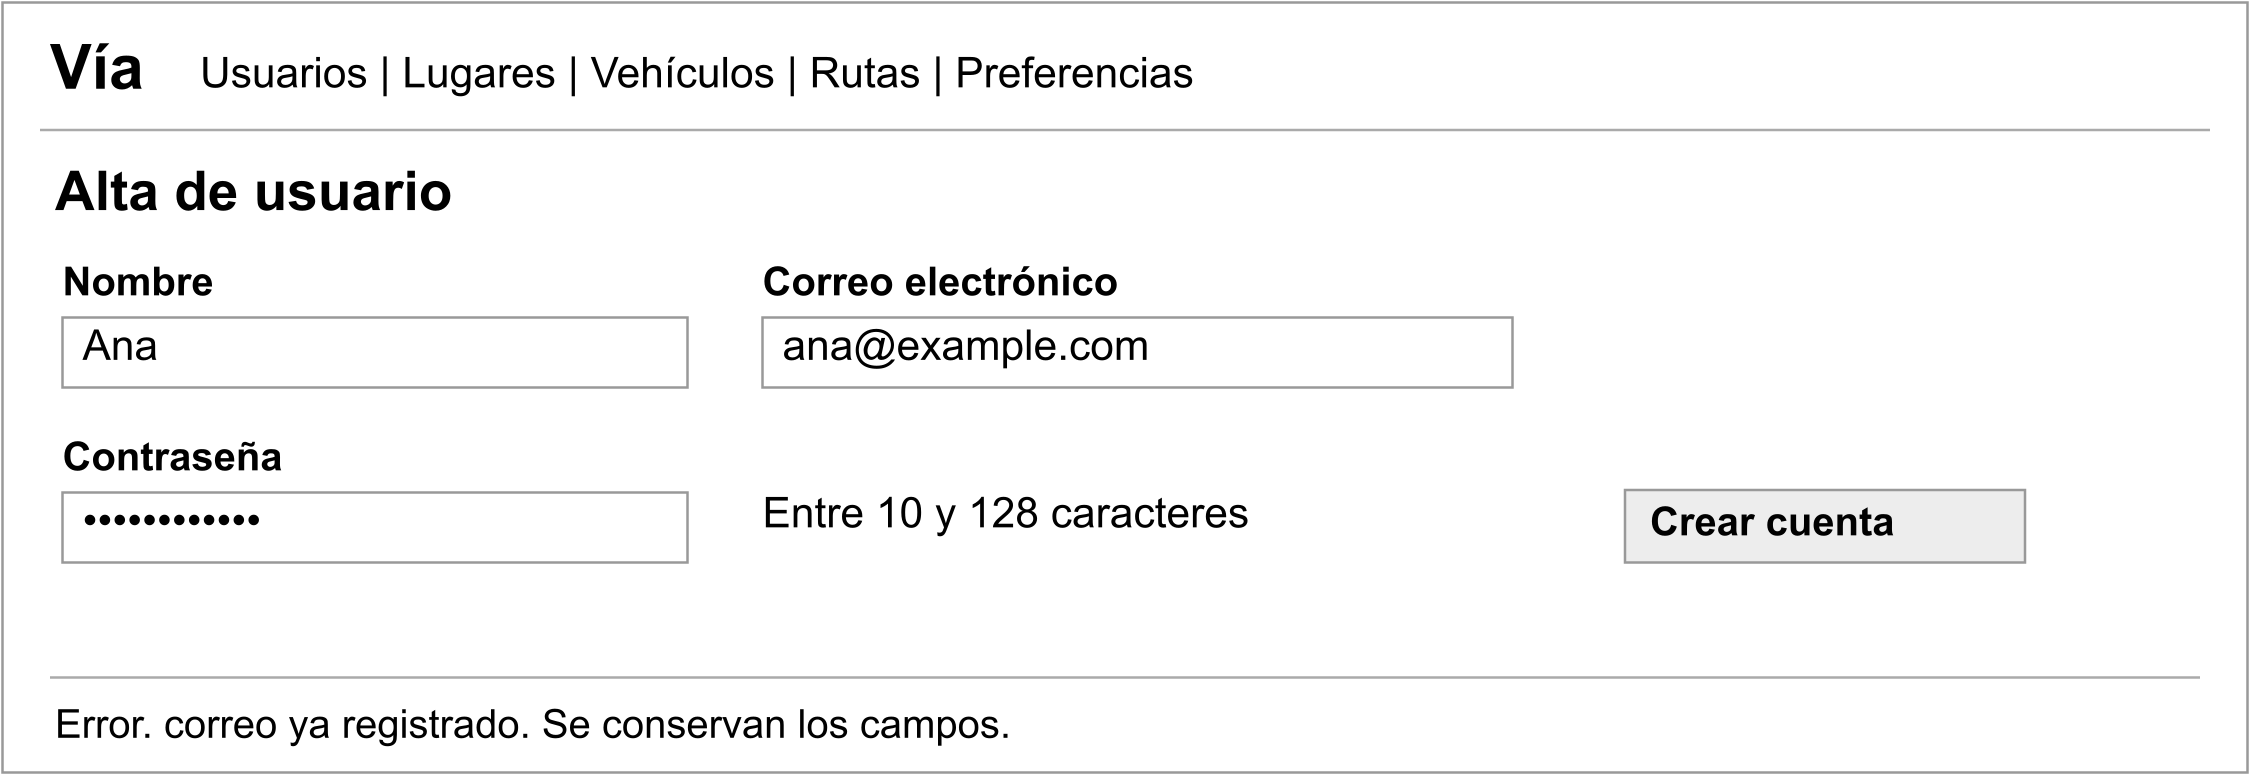
\includegraphics[width=\linewidth]{M01.png}\par
\raggedright{\fontsize{9.5}{12}\selectfont\textbf{M01 Alta de usuario \textperiodcentered{} HU-01}}\end{minipage}\par\vspace{9pt}
\begin{minipage}{\linewidth}\centering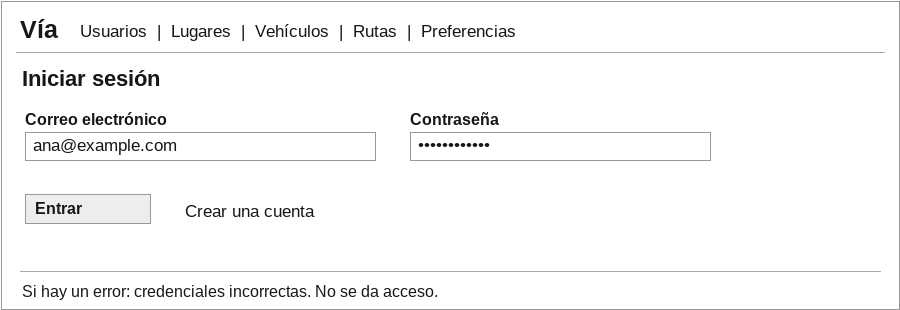
\includegraphics[width=\linewidth]{M02.png}\par
\raggedright{\fontsize{9.5}{12}\selectfont\textbf{M02 Acceso \textperiodcentered{} HU-02}}\end{minipage}\par\vspace{9pt}
\begin{minipage}{\linewidth}\centering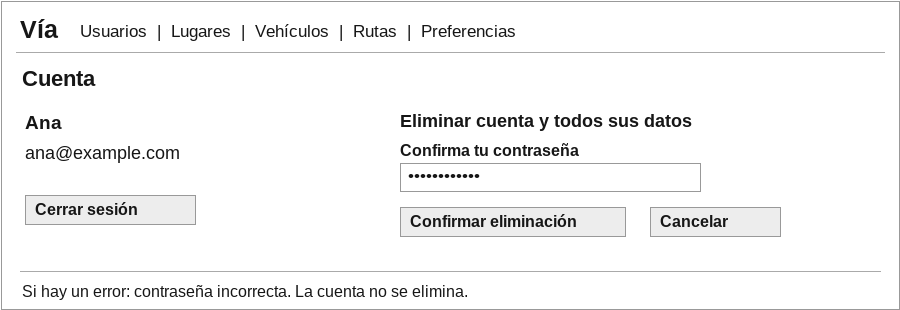
\includegraphics[width=\linewidth]{M03.png}\par
\raggedright{\fontsize{9.5}{12}\selectfont\textbf{M03 Cuenta \textperiodcentered{} HU-03 y HU-04}}\end{minipage}\par\vspace{9pt}
\clearpage
\begin{minipage}{\linewidth}\centering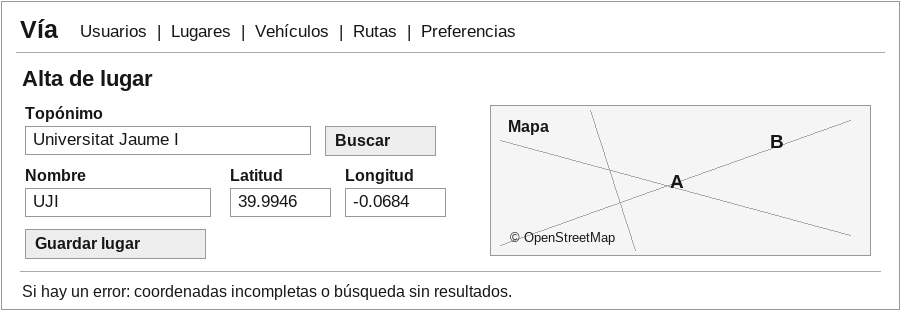
\includegraphics[width=\linewidth]{M04.png}\par
\raggedright{\fontsize{9.5}{12}\selectfont\textbf{M04 Alta de lugar \textperiodcentered{} HU-05, HU-06 y HU-09}}\end{minipage}\par\vspace{9pt}
\begin{minipage}{\linewidth}\centering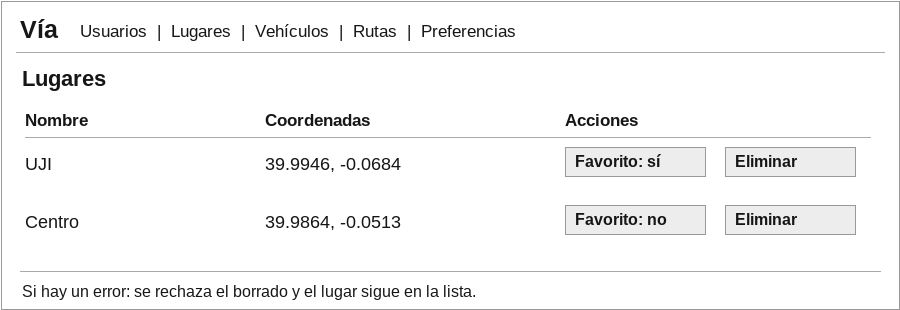
\includegraphics[width=\linewidth]{M05.png}\par
\raggedright{\fontsize{9.5}{12}\selectfont\textbf{M05 Lugares \textperiodcentered{} HU-07, HU-08 y HU-22}}\end{minipage}\par\vspace{9pt}
\begin{minipage}{\linewidth}\centering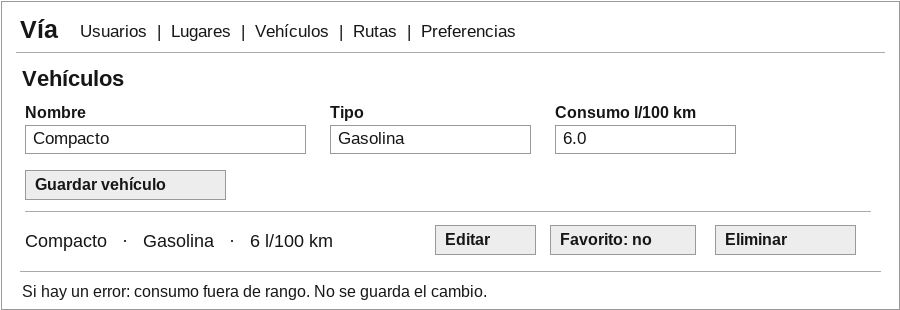
\includegraphics[width=\linewidth]{M06.png}\par
\raggedright{\fontsize{9.5}{12}\selectfont\textbf{M06 Vehículos \textperiodcentered{} HU-10 a HU-13 y HU-22}}\end{minipage}\par\vspace{9pt}
\clearpage
\begin{minipage}{\linewidth}\centering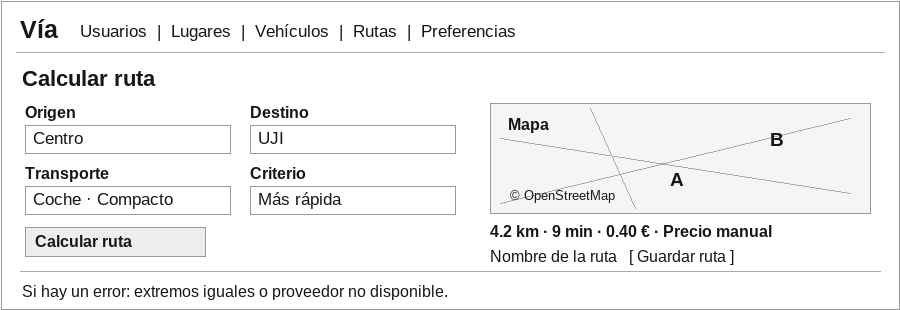
\includegraphics[width=\linewidth]{M07.png}\par
\raggedright{\fontsize{9.5}{12}\selectfont\textbf{M07 Cálculo y resultado \textperiodcentered{} HU-14 a HU-19}}\end{minipage}\par\vspace{9pt}
\begin{minipage}{\linewidth}\centering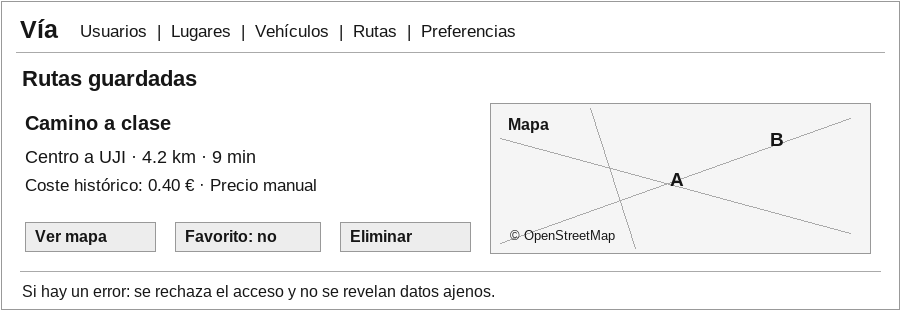
\includegraphics[width=\linewidth]{M08.png}\par
\raggedright{\fontsize{9.5}{12}\selectfont\textbf{M08 Rutas guardadas \textperiodcentered{} HU-20 a HU-22}}\end{minipage}\par\vspace{9pt}
\begin{minipage}{\linewidth}\centering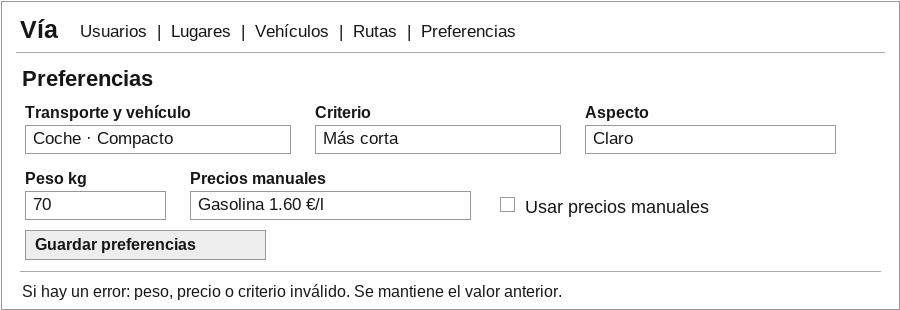
\includegraphics[width=\linewidth]{M09.png}\par
\raggedright{\fontsize{9.5}{12}\selectfont\textbf{M09 Preferencias \textperiodcentered{} HU-23 a HU-26}}\end{minipage}\par\vspace{9pt}
HU-25 y HU-26 se reflejan en la recuperación de las mismas listas y preferencias, sin una pantalla adicional. En móvil el formulario y el mapa se muestran en una sola columna. El mapa tiene una alternativa de entrada por coordenadas.\par
\clearpage
\section{Spike tecnológico}\label{sec5}
El spike integra React y TypeScript en la interfaz, Vite para la compilación, Node.js 24.16 o superior en el servidor, SQLite para el almacenamiento y Leaflet con OpenStreetMap para el mapa. El objetivo es comprobar que estas piezas pueden comunicarse y que los datos guardados se recuperan al volver a abrir la aplicación.\par
La interfaz se suscribe a un modelo de vista observable. Las peticiones HTTP llegan a MobilityService, que coordina los casos de uso. RepositoryPort separa el almacenamiento y RoutingPort, GeocodingPort y PricePort aíslan los servicios externos. Esta separación permite cambiar un proveedor por un doble de prueba sin modificar las pantallas.\par
\begingroup\fontsize{9.25}{11.7}\selectfont\begin{tabularx}{\linewidth}{@{}p{3.2cm}Y@{}}\arrayrulecolor{black}\toprule
\textbf{Servicio} & \textbf{Uso en el spike}\\[3pt]\midrule
\textbf{OpenRouteService} & Geocodificación y rutas en coche, bicicleta y a pie. Clave solo en el servidor.\\[3pt]\arrayrulecolor{black!25}\midrule[0.25pt]
\textbf{OpenStreetMap} & Mapa y selección visual con Leaflet. Se mantiene la atribución.\\[3pt]\arrayrulecolor{black!25}\midrule[0.25pt]
\textbf{MITECO} & Precios de gasolina y diésel como media de las estaciones con datos.\\[3pt]\arrayrulecolor{black!25}\midrule[0.25pt]
\textbf{REE} & Precio eléctrico de referencia. Conversión de \texteuro{}/MWh a \texteuro{}/kWh.\\[3pt]\arrayrulecolor{black!25}\midrule[0.25pt]
\end{tabularx}\endgroup\par
\subsection*{Cálculos y decisiones}
El coste se calcula multiplicando distancia en km / 100 por el consumo medio y por el precio de la energía. El consumo se expresa en l/100 km o kWh/100 km, y el precio en \texteuro{}/l o \texteuro{}/kWh. Para caminar o ir en bicicleta se estiman kcal con MET \ensuremath{\times} 3,5 \ensuremath{\times} peso en kg / 200 \ensuremath{\times} duración en minutos. Se usan MET de 3,5 y 6,8, respectivamente.\par
El criterio económico compara las alternativas recibidas del proveedor. Los criterios de rapidez y distancia pueden devolver la misma opción. Si falta un precio, se muestra el coste como no disponible. Las rutas guardadas conservan el trazado, las métricas y la fuente del cálculo original. En el spike se recuperan los datos confirmados, los favoritos, las preferencias y la selección del último trayecto.\par
\subsection*{Ejecución y resultados}
Desde 02\_Spike se ejecutan npm ci, npm run build y npm run spike. La aplicación se abre en http://localhost:4173. OpenRouteService requiere configurar ORS\_API\_KEY en .env; el resto de proveedores no necesita clave. Los adaptadores mantienen las peticiones externas en el servidor y normalizan sus respuestas antes de utilizarlas en la aplicación.\par
La comprobación local supera 34 pruebas de validación, adaptadores, aislamiento de cuentas y persistencia, además de cuatro recorridos de navegador en Chrome de escritorio y móvil emulado. Estos recorridos comprueban altas, edición, favoritos, cálculo, guardado, recarga, preferencias, cancelación del borrado y tratamiento de errores. Utilizan SQLite en memoria y proveedores de prueba.\par
Las pruebas de persistencia incluyen la reapertura de SQLite y la recuperación de una escritura confirmada tras terminar el proceso con SIGKILL. Este ensayo verifica la caída del proceso, sin simular daños físicos en el almacenamiento. El catálogo contiene 52 especificaciones de aceptación; las comprobaciones automatizadas del spike verifican su viabilidad técnica, no la implementación completa de las historias.\par
\clearpage
\section{Experiencia con Codex}\label{sec6}
Codex se utilizó en distintas fases del trabajo. Primero sirvió para interpretar las instrucciones y distinguir lo que correspondía a la primera entrega de lo que se desarrollará después. La orientación inicial daba demasiado peso a una aplicación completa. La indicación \guillemotleft{}una pantalla por cada funcionalidad\guillemotright{} llevó a acotar el spike y a centrarse en comprobar las conexiones entre sus componentes.\par
Después se trabajó sobre las historias de usuario y sus escenarios. Se mantuvo la separación entre usuarios, lugares, vehículos, rutas, preferencias y persistencia. Los costes de combustible y electricidad se trataron por separado para revisar sus unidades. En los escenarios de rutas se sustituyeron las expectativas de distancia fija por comprobaciones sobre el resultado recibido, porque una API real puede cambiar el trayecto que devuelve.\par
Para el código y las interfaces se conservaron el stack y los adaptadores existentes. Se descartaron el copiloto y las simulaciones porque no eran necesarios para la iteración 0. Las propuestas se comprobaron con pruebas y con el navegador: se corrigieron las etiquetas de los desplegables y un error de Leaflet al cambiar de pantalla durante una animación.\par
La herramienta ayudó a redactar borradores, organizar los escenarios y localizar errores. Su principal inconveniente fue ampliar el alcance más de lo necesario. Además, los datos simulados permiten comprobar cálculos y errores, pero no demuestran que un servicio público esté disponible. Se mantuvo una interfaz sencilla y se distinguieron ambos tipos de prueba. Para las siguientes iteraciones conviene definir primero las pruebas y contrastar las propuestas con el enunciado y con el código.\par
\subsection*{Referencias}
[1] Proyecto conjunto EI1039-EI1048. Descripción, requisitos y herramientas. Curso 2026-2027, versión 1.0.\par
[2] Proyecto conjunto EI1039-EI1048. Metodología y criterios de evaluación. Curso 2026-2027.\par
[3] Entrega 1. Análisis de historias de usuario, diseño de mockups y spike. Material docente, 17 diapositivas.\par
[4] Presentación del proyecto conjunto EI1039-EI1048. Material docente, 31 diapositivas.\par
[5] GAIDeT Declaration Generator. https://panbibliotekar.github.io/gaidet-declaration/ (consulta: 15/10/2026).\par
\subsection*{Declaración GAIDeT}
\begingroup\fontsize{9.25}{11.7}\selectfont
\textbf{Responsables de la delegación:} Ruben Andres Szasz Szasz, Kilian Escudero Vizcaino e Ismael Ferrando Paulo.\par
\textbf{Herramienta y modelo:} Codex de OpenAI, basado en GPT-6.\par
\begin{tabularx}{\linewidth}{@{}p{3.5cm}Y@{}}\arrayrulecolor{black}\toprule
\textbf{Categoría GAIDeT [5]} & \textbf{Tareas delegadas y aplicación en la entrega}\\[3pt]\midrule
\textbf{Desarrollo de software y automatización} & Generación y optimización de código; automatización de procesos. Se aplicó al spike, las interfaces, las pruebas y la compilación del informe.\\[3pt]\arrayrulecolor{black!25}\midrule[0.25pt]
\textbf{Redacción y edición} & Generación de texto, revisión y edición, y cambio de formato. Se aplicó a los borradores de historias, escenarios y memoria, y a su preparación en LaTeX.\\[3pt]\arrayrulecolor{black!25}\midrule[0.25pt]
\textbf{Supervisión} & Evaluación de calidad e identificación de limitaciones. Se aplicó a la coherencia de los escenarios, la detección de errores y la revisión del alcance y de las comprobaciones.\\[3pt]\arrayrulecolor{black!25}\midrule[0.25pt]
\end{tabularx}\par
La IA no asume la autoría ni la responsabilidad del trabajo. La responsabilidad final del contenido corresponde a los tres integrantes indicados.\par
\endgroup
\end{document}
